\section{Introduction}
When studying intelligence, insects, reptiles, and humans have been found to possess neurons with the capacity to hold integer, real numbers, and perform arithmetic operations \cite{nieder-neuronal-number,rugani-arithmetic-chicks,gallistel-numbers-in-brain}.
In our quest to solve intelligence we have put much faith in neural networks, which in turn has provided unparalleled and often superhuman performance in tasks requiring high cognitive ability \cite{natureGo,googleNMT,resnet}.
However, when using neural networks try to learn simple arithmetic problems, such as counting, multiplication, or comparison they systematically fail to extrapolate onto unseen ranges \cite{stillNotSystematic,suzgun2019evaluating,trask-nalu}.

In this paper, we analyze and improve parts of the recently proposed Neural Arithmetic Logic Unit (NALU) \cite{trask-nalu}, which we will introduce in section \ref{sec:Nalu}. Our contributions are; an alternative formulation of the soft weight constraint with a clipped linear activation, parameter regularization that biases towards a sparse solution of $\{-1,0,1\}$, and a reformulation of the multiplication unit with a partial linearity. All of which significantly improves upon the existing $\text{NAC}_{+}$ and $\text{NAC}_{\bullet}$ units as shown through extensive testing on arithmetic constructions.

The NALU is a neural network layer with two sub-units; the $\text{NAC}_{+}$ for addition/subtraction and the $\text{NAC}_{\bullet}$ for multiplication/division.
The sub-units are softly gated between using a sigmoid function. The parameters, which are computed by a soft weight constraint using a tanh-sigmoid transformation, are learned by observing arithmetic input-output pairs and using backpropagation. \cite{rumelhart1986learning}.
\begin{figure}[h]
\centering
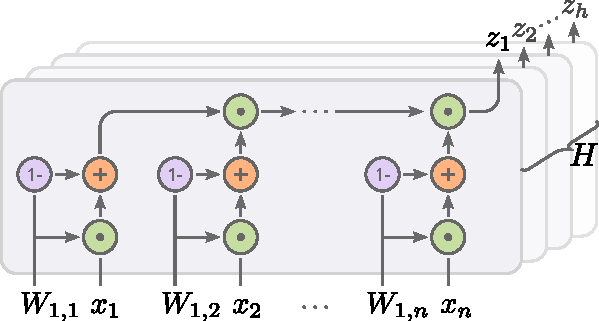
\includegraphics[scale=0.6]{graphics/nmu.pdf}
\caption{Visualization of NMU for a single output scalar $z_1$, this construction repeats for every element in the output vector $\mathbf{z}$.}
\end{figure}
We motivate our work by an investigation of the NALU components; the parameter transformation, the sub-units, $\text{NAC}_{+}$ and $\text{NAC}_{\bullet}$, and the soft gating mechanism.
The investigation uncovers the following analytical and empirical concerns; the gradients from the weight matrix construction in $\text{NAC}_{+}$ and $\text{NAC}_{\bullet}$ have zero expectation, the $\text{NAC}_{\bullet}$ has a treacherous optimization space with unwanted global minimas (as shown in figure \ref{fig:nac-mul-eps-issue}) and has exploding/vanishing gradients, when applying the $\text{NAC}_{+}$ in isolation, we observe that the wanted weight matrix values of $\{-1, 0, 1\}$ are rarely found, and our emperical results reveals that the NALU is significantly worse than hard-choosing either the $\text{NAC}_{+}$ or $\text{NAC}_{\bullet}$, indicating that the gating might not work as intended.

We choose to avoid the gating mechanism as we see no obvious solution to simultaneously train two vastly different operations, the NAU and NMU, with a soft gating mechanism.
We will thus assume that the desired operation is already known, or can empirically be found by varying the network architecture.

%It is fair to assume that the ability to perform arithmetic operations is crucial modern intelligence.
%However, Neural networks(nature, yann lecun), even though it has great expressiveness, has shown an inability to count severe lacks the ability to explicitly only has the ability to has an extreme capacity to interpolate complex functions from simply observing data (ICLR best paper 2017).
%However, even when extrapolating to unseen data we often find a sharp in performance.\cite{missing-cite:image-with-modification}(systematic, nalu, Anders paper).
%Such inability to extrapolate either requires the training distribution to cover the entire distribution (DAGGER) or simply restrics certain systems to be built all together.

%Our solution

%Experiments

%Results





%Remove
%So far, there have not been much research in training exact arithmetic operations for extrapolation. The most important research, is by far, the recently proposed NAC and NALU \cite{trask-nalu}. However, as we will show both analytically and empirically, their results are highly exaggerated, as the proposed arithmetic units are extremely difficult to make convergence consistently. In fact, even without gating mechanism their multiplication operator can't converge on extremely simple problems. For the cases of addition there do converge, a nearly sparse weight matrix of values close to ${-1, 0, 1}$ is rarely found, which also contradicts one of their core claims.
%Motivated by these convergence and sparsity issue, we focus on improving the arithmetic units themself, without considering the gating mechanism in NALU. That is, we will assume that the appropriate operation is already known, or can empirically be found by varying the network architecture which is very common when developing neural networks.